\chapter{Display the Game}

I've chosen the \emph{Simple and Fast Multimedia Library}
\href{https://www.sfml-dev.org/index.php}{SFML} for creating the graphical user interface
of the app.
It lives up to its name and is available on all major platforms and programming languages.

In this chapter we'll learn how to display the board and the chess pieces on it.
In order to show valid moves for each piece, we will also learn the basic rules of the game.

I'm using \href{https://cmake.org/}{CMake} for building the C\textsuperscript{++} code,
and the SFML CMake project template, which will build the SFML libraries.
So you will need to have the following components installed on your machine:

\begin{itemize}
  \item a decent C\textsuperscript{++} compiler (any of the major compilers will do)
  \item the \emph{git} tool
  \item the \emph{cmake} tool
  \item the required system packages for
    \href{https://www.sfml-dev.org/tutorials/2.6/start-cmake.php}{SFML}
\end{itemize}
 
On a linux system, all those components can be installed with your systems package manager
(e.g. with \texttt{apt-get} on Ubuntu).
For Mac OS, just use the included \texttt{clang++} compiler and install
missing components with \href{https://brew.sh/}{homebrew}:
\texttt{<brew install git cmake sfml>}.

When everything is in place, just clone my repository with\\
\texttt{<git clone https://github.com/okrischer/ThinkChess.git>}\\
and execute \texttt{<cmake -B build>} from the root folder of your local copy.\\
If everything went well, change to the \texttt{build} folder and execute \texttt{<cmake --build .>}.\\
Voila, you have a simple chess app, which you can start with \texttt{<./ThinkChess>}.

I strongly encourage you to code all the following steps with an editor of your choice
for yourself and see if you can get the code running. Nothing is gained if you just skim
over the provided source code.

If you have \LaTeX\ installed on your machine, you can also build the documentation
with \texttt{<pdflatex -shell-escape ThinkChess++.tex>} from the \texttt{doc} folder,
which will produce this document.

\section{Displaying the board and the pieces}

Let's start with the basic framework for displaying something with SFML:

\begin{cpp*}{linenos}
#include <SFML/Graphics.hpp>

int main() {
  sf::ContextSettings settings;
  settings.antialiasingLevel = 8;
  auto window = sf::RenderWindow{ {640u, 640u}, "ThinkChess++",
              sf::Style::Default, settings };
  window.setFramerateLimit(10);

  while (window.isOpen()) {
    for (auto event = sf::Event{}; window.pollEvent(event);) {
      if (event.type == sf::Event::Closed) {
        window.close();
      }
    }
    window.draw(bs);
    window.display();
  }
}
\end{cpp*}

This is the main file for our app (\texttt{app/main.cpp}).
Thus, it defines the \mintinline{cpp}{int main()} function (3) as the starting point of the app.
The numbers in paranthesis \texttt{(x)} always refer to the last code snippet.\\
In order to access SFML functionality, we have to \mintinline{cpp}{#include} the SFML Graphics
library (1), which was built by \emph{cmake}.\\
First, we define the context (4) and set the antialiasing level to 8 within the context (5).\\
Next, we define the main window for our app (6), setting its size, title, style, and the context
settings.\\
Then we set the framerate to 10 (8), i.e. 10 frames per second; we don't need more
for such a static app, and the app will keep responsive with that.\\
Next comes the central part: entering the main game loop (10-18). The game loop usually contains
three steps:

\begin{enumerate}
  \item an event loop, processing all user inputs for the current frame (11-15)
  \item several drawing instructions (16) for all items to appear in the frame
  \item a call to \mintinline{cpp}{window.display()}, which causes all drawn elements to be
    actually displayed.
\end{enumerate}

\subsection{The board}
We don't have anything to draw yet; let's change this by adding a chessboard
within the main function, just before entering the game loop:

\begin{cpp*}{linenos}
  sf::Texture bi;
  bi.loadFromFile("../img/chessboard.jpg");
  sf::Sprite bs;
  bs.setTexture(bi);
\end{cpp*}

Here, we create a SFML texture (1) and load an image from the file system into that texture (2).
Then we create a SFML sprite (3) and set its texture  to that image (4).

If you run the app now, you would see an empty chess board:

\begin{center}
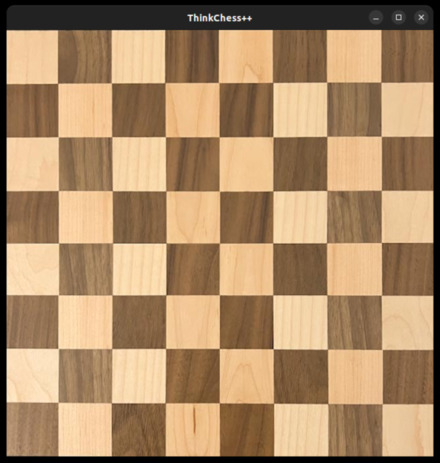
\includegraphics[width=.5\linewidth]{img/emptyBoard.jpg}
\end{center}

\subsection{The pieces}\label{subsec:pieces}
Not that interesting so far, so we're going to add the chess pieces at their initial position.
For that, let's introduce the pieces at first: they come in two colors, \emph{white}
and \emph{black}, each for one player, and they are called as follows
(from left to right in the image below):

\begin{center}

\includegraphics[width=.5\linewidth]{../img/figures.png}
\end{center}

\begin{center}
\begin{tabular}{l | c | c | c | c | c | c}
  \hline
  Piece & King & Queen & Bishop & Knight & Rook & Pawn \\
  quantity & 1 & 1 & 2 & 2 & 2 & 8 \\
  value  & - & 8 & 3 & 3 & 4 & 1 \\
  \hline
\end{tabular}
\end{center}

Every piece, except the king, has a value assigned to it; this is just by convention and
not necessary for the original game play.
The value indicates the strength of the piece and serves for a basic evaluation of each players
position during the game.

The \emph{Queen} is the most powerful piece in the game, followed by the \emph{Rook};
those two are also called \emph{major pieces}.
Then we have the \emph{Bishop} and the \emph{Knight}, both of equal value, building the
group of \emph{minor pieces}.
The least worthy piece is the \emph{Pawn}.

But why has the \emph{King} no value assigned?\\
The goal of the game is to put your opponents \emph{King} in a position, where it is attacked
by any of your own pieces (an attack is the threat to capture a piece with the next move).
We call this position \emph{check}.\\
If a player cannot respond to a \emph{check} in the very next move (i.e. defend his \emph{King}),
the game is over, and that player has lost the game.
We call this position \emph{checkmate}.\\
Thus, the \emph{King} is never actually captured, it stays on the board until the end of the game.
With that, it doesn't make any sense to give it a value for evaluating a players position. 

We'll cover the movement of the pieces in great detail in the next section~\ref{subsec:validmoves}.
But, for now, let's concentrate on how to display the pieces:

\begin{cpp*}{linenos}
  sf::Texture figures;
  figures.loadFromFile("../img/figures.png");

  sf::Sprite wk;
  wk.setTexture(figures);
  wk.setTextureRect(sf::IntRect(0,0,60,60));

  sf::Sprite bk;
  bk.setTexture(figures);
  bk.setTextureRect(sf::IntRect(0,60,60,60));
  // --- snip ---
\end{cpp*}

We have loaded a texture, containing the figures of all pieces (2).
Then we define distinct sprites for every piece, calling them \emph{wk} for the white king (4),
\emph{bk} for the black king (8), and so forth.\\
Finally, we cut out the matching parts of the \mintinline{cpp}{figures} texture and assign
them to every distinct sprite (6, 10).


Notice, that I've taken care that all the sprites have the same size of
$60 \times 60$ pixels.
As the board has a size of $640 \times 640$ pixels, containing $8 \times 8$ light and dark squares,
every square on the board has a size of $80 \times 80$ pixels.
That allows us to place the sprites evenly on the board with an offeset of 10 pixels to the
boundary of each square.

\subsection{Keeping track of the pieces}
In order to actually place the pieces on the board, we need a data structure, being able to
keep track of the 64 squares.
As it turns out, an $8 \times 8$ vector matrix is a good fit for that:

\begin{cpp}
vector<vector<Piece*>> board(8, vector<Piece*>(8));
\end{cpp}

You could have used any type of vector matrix for keeping track of the pieces,
but I've chosen an \emph{object-oriented} approach:
every piece is represented by a raw pointer (indicated with the *) to an instance of the type
\mintinline{cpp}{Piece}.
That allows for greater flexibility implementing the game logic: instead of putting
the logic for the pieces in the main file, we are going to implement it in a new file
\texttt{app/pieces.cpp}.

So, let's have a look on how \mintinline{cpp}{Piece} is actually implemented:

\begin{cpp}
#pragma once
#include <vector>

// public interface for pieces
class Piece {
public:
  virtual ~Piece() {}
  virtual char getType() = 0;
  virtual char getValue() = 0;
  virtual bool isWhite() = 0;
  virtual bool isCaptured() = 0;
  virtual int getRow() = 0;
  virtual int getCol() = 0;
  virtual void capture() = 0;
  virtual bool isValid(std::vector<std::vector<Piece*>>& bd,
                       int r, int c) = 0;
};
\end{cpp}

As you may have guessed, this code snippet is not from the \texttt{pieces.cpp} file, but from its
\emph{header} file, located at \texttt{include/pieces.hpp}.
I've decided to separate the compilation units into a public interface (the header file) and
an implementation file.
That allows to use the definitions of the header file in any other implementation file and
gives us even more flexibility in structuring the source code.

\mintinline{cpp}{Piece} is declared as a pure \emph{abstract} interface.
That means, it doesn't have a \emph{constructor}, and all the member functions are marked
as \mintinline{cpp}{virtual}.
Thus, you cannot instanciate it directly, and to make any use of it, we have to create
\emph{derived} classes (subclasses of \mintinline{cpp}{Piece}) for every piece, which will
implement the virtual functions.
The reason for doing so is: we need different implementations for performing moves for
each piece, but also a common type for storing them in the board matrix. 

The concrete types for \mintinline{cpp}{Piece} are implemented like so:

\begin{cpp*}{linenos}
class King : public Piece {
public:
  ~King() {}
  King(bool w, int r, int c) : type{'K'}, white{w}, value{0},
                              captured{false}, row{r}, col{c} {}

  char getType() override { return type; }
  char getValue() override { return value; }
  bool isWhite() override { return white; }
  bool isCaptured() override { return captured; }
  int getRow() override { return row; }
  int getCol() override { return col; }
  bool isValid(std::vector<std::vector<Piece*>>& bd, int r, int c)
    override;

private:
  char type;
  bool white;
  short value;
  bool captured;
  int row;
  int col;
};
\end{cpp*}

The other pieces are implemented likewise; the only difference between them so far is the
implementation of the member function \mintinline{cpp}{isValid} (13).
I decided to leave all the class definitions in the header file, and moved only the
implementation for \mintinline{cpp}{isValid} to the file \texttt{app/pieces.cpp}.
We'll study these implementations in the next section~\ref{subsec:validmoves}.

For now, we are only interested in the type definitions:\\
each of them is derived from \mintinline{cpp}{class Piece} (1) and has a \emph{destructor} (3),
which will be called by the compiler when an instance of the class is destroyed.
This will happen automatically, whenever an \emph{automatic} variable gets out of scope.
But, if a reference to an instance was created explicitly (using the keyword \mintinline{cpp}{new}),
we have to \mintinline{cpp}{delete} that object explicitly in order to avoid \emph{memory leaks}.

Next, we have the \emph{constructor} (4-5):\\
it initializes a new instance with its type (which we need only for drawing the correct sprite),
the color of the piece (white or black), its value, and the current position
of the piece (the row and column of the piece in the board matrix).

The following member functions (7-12) are just \emph{getters} to retrieve the
\mintinline{cpp}{private} member types.

With the derived \mintinline{cpp}{Piece} types in place, we can initially fill the board matrix:

\begin{cpp}
void reset_board(vector<vector<Piece*>>& bd) {
  for (auto rank : bd) {
    for (auto piece : rank) {
      delete piece;
    }
  }
  // rank 8 (black)
  bd[0][0] = new Rook(0,0,0);
  bd[0][1] = new Knight(0,0,1);
  bd[0][2] = new Bishop(0,0,2);
  bd[0][3] = new Queen(0,0,3);
  bd[0][4] = new King(0,0,4);
  bd[0][5] = new Bishop(0,0,5);
  bd[0][6] = new Knight(0,0,6);
  bd[0][7] = new Rook(0,0,7);
  // rank 7 (black)
  bd[1][0] = new Pawn(0,1,0);
  bd[1][1] = new Pawn(0,1,1);
  bd[1][2] = new Pawn(0,1,2);
  bd[1][3] = new Pawn(0,1,3);
  bd[1][4] = new Pawn(0,1,4);
  bd[1][5] = new Pawn(0,1,5);
  bd[1][6] = new Pawn(0,1,6);
  bd[1][7] = new Pawn(0,1,7);
  // rank 2 (white)
  bd[6][0] = new Pawn(1,6,0);
  bd[6][1] = new Pawn(1,6,1);
  bd[6][2] = new Pawn(1,6,2);
  bd[6][3] = new Pawn(1,6,3);
  bd[6][4] = new Pawn(1,6,4);
  bd[6][5] = new Pawn(1,6,5);
  bd[6][6] = new Pawn(1,6,6);
  bd[6][7] = new Pawn(1,6,7);
  // rank 1 (white)
  bd[7][0] = new Rook(1,7,0);
  bd[7][1] = new Knight(1,7,1);
  bd[7][2] = new Bishop(1,7,2);
  bd[7][3] = new Queen(1,7,3);
  bd[7][4] = new King(1,7,4);
  bd[7][5] = new Bishop(1,7,5);
  bd[7][6] = new Knight(1,7,6);
  bd[7][7] = new Rook(1,7,7);
}
\end{cpp}

That seems tedious, but thankfully we have to do this only once.
I've placed the initialization code within a function \mintinline{cpp}{void reset_board()},
just in case we want to reset the board later (e.g. when starting a new game).
The board is passed as an automatic reference to the function (indicated by the \& after the
parameter type), such that we are able to modify the board directly,
instead of working with a copy of the board.

The code in the first three lines actually resets the board by deleting all existing
references to pieces.
When setting the pieces, you have to be careful: every piece must be initialized with exactly the
same coordinates from the board (and of course with the correct color: 0 for black and 1 for white).

The rows of a chessboard are called \emph{ranks}, while the colums are called
\emph{files}.
The ranks are indicated by the numbers 1 to 8, whereas the files are indicated by the letters
\texttt{a} to \texttt{h}, both starting at the lower left square (the dark field \texttt{a1}):
\begin{samepage}
\begin{verbatim}
8 . . . . . . . .
7 . . . . . . . .
6 . . . . . . . .
5 . . . . . . . .
4 . . . . . . . .
3 . . . . . . . .
2 . . . . . . . .
1 . . . . . . . .
  a b c d e f g h
\end{verbatim}

With the initialization code above, the pieces will be placed like so on the board:

\begin{verbatim}
8 R N B Q K B N R
7 P P P P P P P P
6 . . . . . . . .
5 . . . . . . . .
4 . . . . . . . .
3 . . . . . . . .
2 P P P P P P P P
1 R N B Q K B N R
  a b c d e f g h
\end{verbatim}
\end{samepage}

Observe that we abbreviate the \emph{Knight} with the letter \texttt{N} to avoid confusion with
the \emph{King}.
So, the white \emph{Queen} is placed at \texttt{d1}, the black \emph{Queen} at \texttt{d8},
and so forth.

\subsection{Drawing the pieces}
Now we can use the filled board matrix to actually draw the pieces within the game loop of the
main function:

\begin{cpp*}{linenos}
    // draw board
    window.draw(bs);
    // draw pieces
    for (int row = 0; row < 8; row++) {
      for (int col = 0; col < 8; col++) {
        if (board[row][col]) {
          auto piece = board[row][col];
          sf::Sprite pc;
          switch (piece->getType()) {
          case 'K':
            piece->isWhite() ? pc = wk : pc = bk;
            break;
          case 'Q':
            piece->isWhite() ? pc = wq : pc = bq;
            break;
          case 'R':
            piece->isWhite() ? pc = wr : pc = br;
            break;
          case 'B':
            piece->isWhite() ? pc = wb : pc = bb;
            break;
          case 'N':
            piece->isWhite() ? pc = wn : pc = bn;
            break;
          case 'P':
            piece->isWhite() ? pc = wp : pc = bp;
            break;
          }
          pc.setPosition(col*80.f + 10.f, row*80.f + 10.f);
          window.draw(pc);
        }
      }
    }
\end{cpp*}

We are iterating over all elements of the board matrix and get the piece at this position (7).
Then we get the type and color of that piece by calling the appropriate getter functions
(\mintinline{cpp}{getType(), isWhite()}) on it, and let a newly created sprite \texttt{pc}
point to the corresponding figure sprite (9-28).
Finally, we set the correct postion of the \texttt{pc} sprite on the board (29) and draw it
to the current frame buffer (30).
Observe that we have to use the pointer notation \texttt{->} (instead of a dot) for calling
those functions on a piece, as the pieces were actually defined as pointers.

And that's it: when you start the app now, you will see this screen, which shows a
correct initialized chessboard with all pieces:

\begin{center}
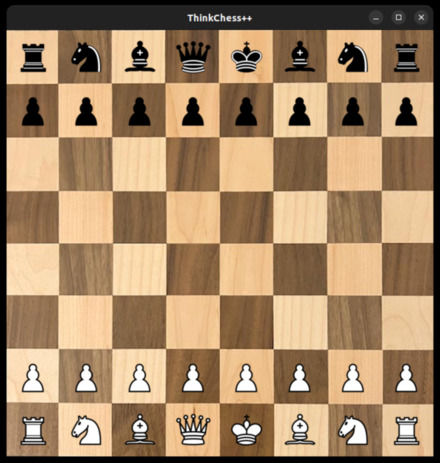
\includegraphics[width=.5\linewidth]{img/boardWithPieces.jpg}
\end{center}


\section{Showing valid moves}\label{sec:validmoves}
The goal for this section is to show the valid moves for any given piece on the board.
\subsection{Game mechanics}

For reaching our goal, we first need a way to process user input.
With SFML this is done inside the event loop of the main function:

\begin{cpp*}{linenos}
      // in event loop
      // mouse button pressed
      if (event.type == sf::Event::MouseButtonPressed) {
        if (event.mouseButton.button == sf::Mouse::Right) {
          pair<int, int> f =
            getField(event.mouseButton.x, event.mouseButton.y);
          setValidMoves(board, board[f.first][f.second]);
        }
      }
      // mouse button released
      if (event.type == sf::Event::MouseButtonReleased) {
        if (event.mouseButton.button == sf::Mouse::Right) {
          validMoves =
            vector<vector<short>>(8, vector<short>(8, 0));
        }
      }
\end{cpp*}

Here, we check if a mouse button is pressed (3).
If so, we check wether it's the right mouse button (4).
Then, we get the coordinates of the corresponding field on the board (5-6), and
fill another vector matrix with the computed valid moves for the piece under the
mouse cursor (7).

When the right mouse button is released (11-12), we reset the vector matrix of
valid moves (13-14).

In order for that to work, we need the following definitions in the main file,
just before entering the main function:

\begin{cpp*}{linenos}
vector<vector<short>> validMoves(8, vector<short>(8, 0));

void setValidMoves(vector<vector<Piece*>>& bd, Piece* pc) {
  if (!pc) return;
  for (int row = 0; row < 8; row++) {
    for (int col = 0; col < 8; col++) {
      if (pc->isValid(bd, row, col)) {
        auto current = bd[row][col];
        if (!current) validMoves[row][col] = 1; 
        else if (pc->isWhite() != current->isWhite())
          validMoves[row][col] = 2;
      }
    }
  }
}

pair<int, int> getField(int x, int y) {
  int fx = x / 80;
  int fy = y / 80;
  auto field = make_pair(fy, fx);
  return field;
}

\end{cpp*}

The work is done inside the \mintinline{cpp}{setValidMoves} function (3):\\
if there's no piece at the given coordinates, do nothing (4).
Otherwise, iterate over all fields of the board (5-6), and check wether this position can be
reached by the piece under the mouse cursor (7).
If so, get the piece of the current search position (8).
If there is no piece at this position, set this position to valid (9).
Otherwise, check the color of the current piece and if it's different from the piece
under the cursor (i.e. it can be captured), set it to valid with the special marker 2 (11).

Our \emph{object-oriented} design is starting to pay off, as we don't need to define any
game logic inside the main application file!

The last thing to do, is to draw the content of the \mintinline{cpp}{validMoves}
vector inside the main game loop (directly after drawing the pieces):

\begin{cpp*}{linenos}
  // before game loop
  sf::CircleShape valid(20.f);

    // inside game loop
    // draw valid moves
    for (int row = 0; row < 8; row++) {
      for (int col = 0; col < 8; col++) {
        if (validMoves[row][col] > 0) {
          valid.setPosition(col*80.f + 20.f, row*80.f + 20.f);
          if (validMoves[row][col] > 1)
            valid.setFillColor(sf::Color(0, 200, 0, 200));
          else valid.setFillColor(sf::Color(100, 200, 0, 100));
          window.draw(valid);
        }
      }
    }
\end{cpp*}

We iterate over all fields of the board (6-7), and if \mintinline{cpp}{validMoves} contains
an entry at this position (8), we set the marker \mintinline{cpp}{valid} on the board (9).
As an extra feature, we set the marker to a brighter color, if the piece at this postion can be
captured (10-11).
Finally, we draw the marker on the board (13).

With that, all valid moves for a selected piece are displayed while pressing the right mouse button
(with a green circular shape on the board). As soon as you release the mouse botton, the
\mintinline{cpp}{validMoves} vector is reset, and there's nothing more to draw for the next frame.

That's all for the mechanics of the game for now. Of course, we still need to implement the
\mintinline{cpp}{isValid} function for every piece, which leads us to the next section.

\subsection{Movement of the pieces}\label{subsec:validmoves}
\subsubsection{The King}

Let's start with the \emph{King}: it can move one step in any direction (on ranks, files and
diagonals), provided the target field is not occopied by a piece of the same color:

\begin{center}
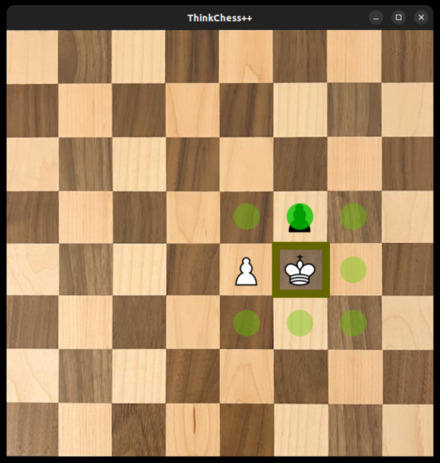
\includegraphics[width=.5\linewidth]{img/king.jpg}
\end{center}

Observe, that the piece, for which the valid moves are shown (the king on \texttt{f4}), is marked
with a dark green frame.
We will learn how to set this marker in section~\ref{sec:makemoves}, so when progamming along,
you will not see this marker for now.

If the target field is occopied by a piece of the other color (the black pawn on \texttt{f5}),
the king can capture that piece, indicated by a brighter color of the green marker.

But notice: the king is the only piece on the board that is not allowed to move to a field,
where it is immediately attacked, as it would put
itself into a \emph{check} position, and the game would be over.
We're not taking this special case into account yet, so the field \texttt{g4},
which is attacked by the black pawn, is still marked as valid.

Besides that, there's also a special move involving the king, called \emph{castling},
which we will cover in section~\ref{sec:specmoves}.

The function \mintinline{cpp}{isValid} for the king is implemented in the file
\texttt{app/pieces.cpp}:

\begin{cpp*}{linenos}
#include "pieces.hpp"
#include <vector>
using namespace std;

bool King::isValid(const vector<vector<Piece*>>& bd, int r, int c) {
  bool valid = abs(r-row) <= 1 && abs(c-col) <= 1;
  return valid;
}
\end{cpp*}

First, we have to include the header file located at \texttt{include/pieces.hpp} (1),
in order to make the type definitions of the pieces available.
Observe, that we don't have to spell out the complete path to that file, thanks to these
instructions of our \texttt{CMakeLists.txt} file:

\begin{cpp}
add_executable(ThinkChess app/main.cpp app/pieces.cpp)
target_include_directories(ThinkChess PUBLIC include)
\end{cpp}

The function \mintinline{cpp}{isValid} is actually defined as
\mintinline{cpp}{King::isValid} (5), which defines the function as a member function of the
type \mintinline{cpp}{King}.
It returns \mintinline{cpp}{true} only if the given coordinates can be reached within one step.

\subsubsection{The Knight}
The \emph{Knight} is also a very special piece in one sense: it is the only piece, able to
jump over any other piece on the board.
It can move like so: either two fields on a rank and one on a file, or two on a file and one on
a rank.
That leads to an L shape for every move:

\begin{center}
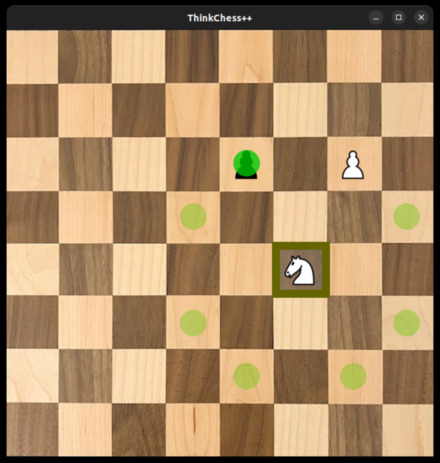
\includegraphics[width=.5\linewidth]{img/knight.jpg}
\end{center}

Observe that a knight, placed on a dark field, can reach only light fields, and vice versa.

Its \mintinline{cpp}{isValid} function is implemented like so:

\begin{cpp}
bool Knight::isValid(const vector<vector<Piece*>>& bd, int r, int c) {
  bool valid = (abs(r-row) == 1 && abs(c-col) == 2) ||
               (abs(r-row) == 2 && abs(c-col) == 1);
  return valid;
}
\end{cpp}

\subsubsection{The Rook}
The \emph{Rook} moves any distance on its current rank or file, but cannot jump over any other piece.

\begin{center}
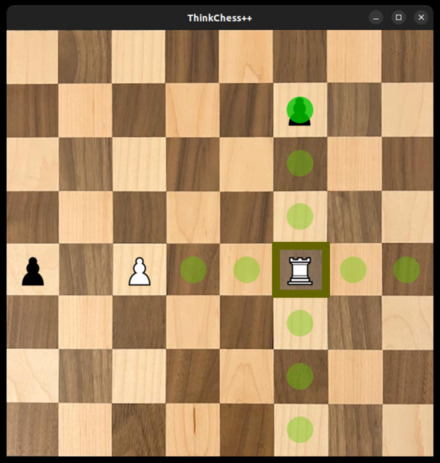
\includegraphics[width=.5\linewidth]{img/rook.jpg}
\end{center}

As the rooks movement is limited by other pieces on its way, we have to take those pieces
into account for implementing its \mintinline{cpp}{isValid} function:

\begin{cpp*}{linenos}
bool Rook::isValid(const vector<vector<Piece*>>& bd, int r, int c) {
  bool valid = r == row || c == col;
  if (r == row && abs(c-col) > 1) { // same row
    if (c < col) { // left
      for (int cc = c+1; cc < col; cc++) {
        auto pc = bd[r][cc];
        if (pc) { valid = false; break; }
      }
    } else { // right
      for (int cc = col+1; cc < c; cc++) {
        auto pc = bd[r][cc];
        if (pc) { valid = false; break; }
      }
    }
  }
  if (c == col && abs(r-row) > 1) { // same column
    if (r < row) { // top
      for (int rr = r+1; rr < row; rr++) {
        auto pc = bd[rr][c];
        if (pc) { valid = false; break; }
      }
    } else { // down
      for (int rr = row+1; rr < r; rr++) {
        auto pc = bd[rr][c];
        if (pc) { valid = false; break; }
      }
    }
  }
  return valid;
}
\end{cpp*}

First, we set the result to \mintinline{cpp}{valid} if the given field it is on the same row
or column as the rook(2).\\
Then, we check for two cases:
\begin{itemize}
  \item the field is on the same row (3), or
  \item the field is on the same column (16).
\end{itemize}

In both cases, we check wether there is another piece between the field and the rook by
iterating over all those fields on that row, respective column.
If so, we set \mintinline{cpp}{valid} to \mintinline{cpp}{false} and stop the search (7, 12, 20, 25).

We have four searches, for every direction the rook can move: up, down, left, right.
But only one of them will ever be executed for any given field: either on the same row \emph{or}
on the same column.
As the search-space is very small for each search (at most 6 checks), we can consider this as a
\emph{constant time} search, or in asymptotic notation $\mathcal{O}(1)$.

\subsubsection{The Bishop}
The \emph{Bishop} can move any distance along the diagonals, on which it is placed,
unless its way is blocked by another piece:

\begin{center}
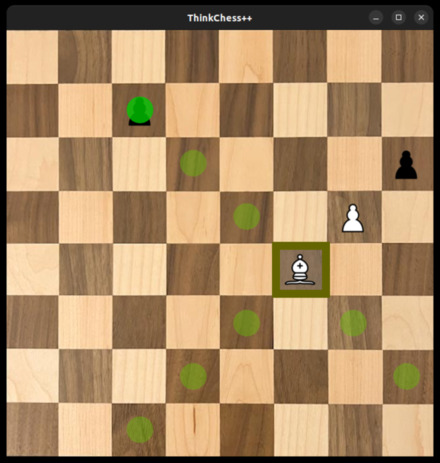
\includegraphics[width=.5\linewidth]{img/bishop.jpg}
\end{center}

Notice, that a bishop, placed initially on a light field, will always stay on a light field,
and vice versa.
Thus, both players each have a \emph{dark} and a \emph{light} bishop (the white bishop on
\texttt{f4} is a \emph{dark} bishop with its initial position on \texttt{c1}).
Dark and light bishops can never attack each other.

We use essentially the same logic as for the rook, but this time we check for pieces on
the same diagonal:

\begin{cpp}
bool Bishop::isValid(const vector<vector<Piece*>>& bd, int r, int c) {
  bool valid = r-c == row-col || r+c == row+col;
  if (r-c == row-col) { // same major diagonal
    if (r < row) { // upper
      for (int rr = row-1; rr > r; rr--) {
        for (int cc = col-1; cc > c; cc--) {
          if (rr-cc == row-col) {
            auto pc = bd[rr][cc];
            if (pc) { valid = false; break; }
          }
        }
      }
    } else { // lower
      for (int rr = row+1; rr < r; rr++) {
        for (int cc = col+1; cc < c; cc++) {
          if (rr-cc == row-col) {
            auto pc = bd[rr][cc];
            if (pc) { valid = false; break; }
          }
        }
      }
    }
  }
  if (r+c == row+col) { // same minor diagonal
    if (r < row) { // upper
      for (int rr = row-1; rr > r; rr--) {
        for (int cc = col+1; cc < c; cc++) {
          if (rr+cc == row+col) {
            auto pc = bd[rr][cc];
            if (pc) { valid = false; break; }
          }
        }
      }
    } else { // lower
      for (int rr = row+1; rr < r; rr++) {
        for (int cc = col-1; cc > c; cc--) {
          if (rr+cc == row+col) {
            auto pc = bd[rr][cc];
            if (pc) { valid = false; break; }
          }
        }
      }
    }
  }
  return valid;
}
\end{cpp}

Here, we also have four searches: two for the major diagonal and another two for the minor
diagonal.
The searches are now nested loops, as we need to get both coordinates for the current field.
There are at most $6 \times 6 = 36$ tests per search, and on average only $3 \times 3 = 9$
tests for each.
And, as before, only one of these searches will ever by executed for any given field.
So, we may consider these searches as \emph{constant time} searches as well.

\subsubsection{The Queen}
The \emph{Queen} can move any distance in all directions (on its rank, file or diagonals),
only limited by other pieces in its way.
In the image below you can see, why the queen is the strongest piece on the board:

\begin{center}
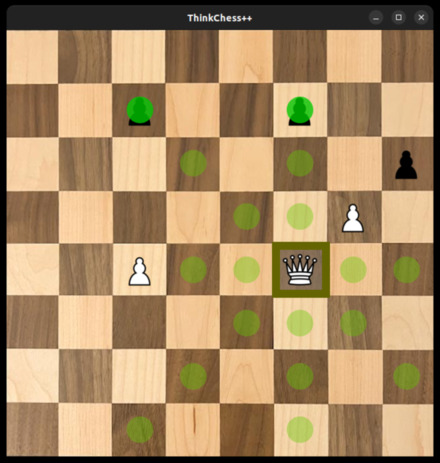
\includegraphics[width=.5\linewidth]{img/queen.jpg}
\end{center}

We use a little trick to get the queens valid moves: as the queen can move like a rook
\emph{and} a bishop, we just check for valid moves for \emph{either} of them:

\begin{cpp}
bool Queen::isValid(const vector<vector<Piece*>>& bd, int r, int c) {
  auto rook = new Rook(white, row, col);
  auto bishop = new Bishop(white, row, col);
  bool valid = rook->isValid(bd, r, c) || bishop->isValid(bd, r, c);
  delete rook;
  delete bishop;
  return valid;
}
\end{cpp}

Observe that we have to delete those dummy pieces, in order to prevent any memory leaks.

\subsubsection{The Pawn}
The last piece to cover is the \emph{Pawn}: it is the weakest piece on the board, but in
exchange, both players have 8 of them.
The movement of the pawns is the most complex of all pieces:

\begin{itemize}
  \item \textbf{base case}: move straight forward one square on its file, if that square is vacant
  \item \textbf{capturing}: capture an opponents piece on eiher of the two squares diagonally
    in front of it
  \item \textbf{initial position}: if the pawn has not yet moved, it has the option of moving two
    squares straight forward, provided both squares are vacant.
\end{itemize}

Notice that the terms \emph{forward} and \emph{in front} always refer to the direction towards
the opponents pieces: the \emph{white} pawns moves to the higher ranks (e.g. \texttt{e2-e4}),
while the \emph{black} pawns move towards the lower ranks (e.g. \texttt{d3xe2}).

\begin{center}
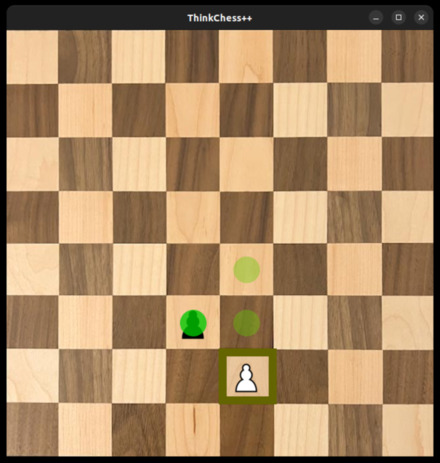
\includegraphics[width=.5\linewidth]{img/pawn.jpg}
\end{center}

There are also two special moves involving pawns, called \emph{en passant} and \emph{promotion},
which we will cover in section~\ref{sec:specmoves}.

Here's the code to put the rules in action:

\begin{cpp*}{linenos}
bool Pawn::isValid(const vector<vector<Piece*>>& bd, int r, int c) {
  bool valid = false;
  auto pc = bd[r][c];
  if (white) {
    if (r == row-1 && c == col) { // move
      if (!pc) valid = true;
    }
    if (row == 6 && r == 4 && c == col) { // initial move
      auto pc1 = bd[5][c];
      if (!pc1 && !pc) valid = true;
    }
    if (r == row-1 && (c == col-1 || c == col+1)) { // capture
      if (pc && pc->isWhite() != white) valid = true;
    }
  } else { // black
    if (r == row+1 && c == col) { // move
      if (!pc) valid = true;
    }
    if (row == 1 && r == 3 && c == col) { // initial move
      auto pc1 = bd[2][c];
      if (!pc1 && !pc) valid = true;
    }
    if (r == row+1 && (c == col-1 || c == col+1)) { // capture
      if (pc && pc->isWhite() != white) valid = true;
    }
  }
  return valid;
}
\end{cpp*}

We have to consider white and black pawns separately, as they move in different directions (4, 15).
If there's no piece in front of the pawn, it can move to that field (6, 17).
If the pawn is on its initial position (8, 19), it also can move two squares ahead, if both fields
ahead aren't occopied (10, 24).
If there's a piece diagonal in front of the pawn (12, 23), it can be captured, if it is of the
other color (13, 24).
